\documentclass{beamer}
\usepackage[utf8]{inputenc}
\usepackage[spanish]{babel}

\usepackage{latexsym,amsmath,xcolor,bm, amssymb, color, tikz, graphicx, amsthm, mathtools}
\usepackage{algorithm}
\usepackage{algorithmic}
\usepackage{hyperref}
\usepackage{float}     
\usepackage{CJKutf8}
\usepackage{multicol}
\usepackage{pgf-pie}

\graphicspath{{../logos/}{img/}}

\DeclareMathOperator*{\argmax}{arg\,max}
\DeclareMathOperator*{\argmin}{arg\,min}
\DeclareMathOperator{\sign}{sign}
\DeclareMathOperator{\Tr}{Tr}

\makeatletter
\DeclareRobustCommand\onedot{\futurelet\@let@token\@onedot}
\def\@onedot{\ifx\@let@token.\else.\null\fi\xspace}
\def\eg{\emph{e.g}\onedot} 
\def\Eg{\emph{E.g}\onedot}
\def\ie{\emph{i.e}\onedot} 
\def\Ie{\emph{I.e}\onedot}
\def\cf{\emph{c.f}\onedot} 
\def\Cf{\emph{C.f}\onedot}
\def\etc{\emph{etc}\onedot} 
\def\vs{\emph{vs}\onedot}
\def\wrt{w.r.t\onedot} 
\def\dof{d.o.f\onedot}
\def\etal{\emph{et al}\onedot}
\makeatother

\usetheme{Madrid}
\useinnertheme{circles}

% Theme color: UNLP Bordeaux
\definecolor{ColorUNLP}{HTML}{8c0011} 
\usecolortheme[named=ColorUNLP]{structure}

%------------------------------------------------------------
% Info de la presentación
\title{Cierre Training Camp Argentina 2026}
\subtitle{Ceremonia de Clausura}
\author[AAPC]{Asociación Argentina de Programación Competitiva}
\institute[]{Universidad Nacional de La Plata -- Facultad de Informática}
\date[TC 2026]{Training Camp 2026}
\titlegraphic{
\includegraphics[clip,height=2cm,keepaspectratio]{logoTC.pdf}}
%------------------------------------------------------------

\AtBeginSection[]
{
  \begin{frame}
    \frametitle{Temario}
    \tableofcontents[currentsection]
  \end{frame}
}

\begin{document}

\frame{\titlepage}

% --- Sponsors Frame (2026 formats & logos) ---
\begin{frame}{Gracias Sponsors!}
    \begin{columns}[t]
        \column{0.5\textwidth}
        \centering
        Organiza\\
        \vspace{0.5cm}
        
\includegraphics[width=0.6\textwidth,keepaspectratio]{logo_aapc.png}\\
        \vspace{0.3cm}
        
\includegraphics[width=0.8\textwidth,keepaspectratio]{unlp_informatica.png}
        \column{0.5\textwidth}
        \centering
        Diamond Sponsor\\
        \vspace{0.5cm}
        
\includegraphics[width=0.8\textwidth,keepaspectratio]{GTSlogo.jpeg}
    \end{columns}
\end{frame}

\section{Gracias por venir}

% % TODO: Update participant counts on the final day
\begin{frame}{Participantes por País}
\begin{center}
\Large
\textbf{¡215 participantes presentes!}

\vspace{0.4cm}

\normalsize
\textbf{Distribución por países:}

\vspace{0.3cm}

\begin{columns}[t]
\column{0.5\textwidth}
\begin{itemize}
\item \textbf{Argentina:} 121
\item \textbf{Chile:} 16
\item \textbf{Perú:} 15
\item \textbf{Bolivia:} 14
\item \textbf{México:} 13
\item \textbf{Costa Rica:} 12
\end{itemize}
\column{0.5\textwidth}
\begin{itemize}
\item \textbf{Uruguay:} 12
\item \textbf{Colombia:} 6
\item \textbf{Brasil:} 2\textsuperscript{*}
\item \textbf{Ecuador:} 2
\item \textbf{Venezuela:} 1
\item \textbf{El Salvador:} 1
\end{itemize}
\end{columns}

\vspace{0.3cm}
\footnotesize{\textsuperscript{*} Representando a la UNLP}
\end{center}
\end{frame}

\begin{frame}{Diversidad Regional}
\begin{center}
\Large
\textbf{12 países representados}

\vspace{0.3cm}

\begin{tikzpicture}[scale=0.9]
  % Argentina
  \fill[blue,opacity=0.7] (3.2,1.1) circle (0.26);
  \node[left] at (2.9,1.1) {\textbf{Argentina} (121)};
  % Uruguay
  \fill[cyan,opacity=0.7] (3.7,1.3) circle (0.11);
  \node[right] at (3.8,1.3) {Uruguay (12)};
  % Chile
  \fill[green,opacity=0.7] (2.2,1.7) circle (0.12);
  \node[left] at (2.0,1.7) {Chile (16)};
  % Bolivia
  \fill[teal,opacity=0.7] (2.7,2.3) circle (0.12);
  \node[right] at (2.8,2.3) {Bolivia (14)};
  % Peru
  \fill[red,opacity=0.7] (2.0,3.0) circle (0.12);
  \node[left] at (1.8,3.0) {Perú (15)};
  % Brasil
  \fill[yellow,opacity=0.7] (4.1,3.2) circle (0.08);
  \node[right] at (4.2,3.2) {Brasil (2)};
  % Ecuador
  \fill[pink,opacity=0.7] (1.8,3.8) circle (0.08);
  \node[left] at (1.6,3.8) {Ecuador (2)};
  % Colombia
  \fill[violet,opacity=0.7] (2.0,4.5) circle (0.09);
  \node[left] at (1.8,4.5) {Colombia (6)};
  % Venezuela
  \fill[magenta,opacity=0.7] (2.8,4.8) circle (0.07);
  \node[right] at (2.9,4.8) {Venezuela (1)};
  % Costa Rica
  \fill[orange,opacity=0.7] (1.3,5.2) circle (0.11);
  \node[left] at (1.1,5.2) {Costa Rica (12)};
  % El Salvador
  \fill[olive,opacity=0.7] (1.0,5.8) circle (0.07);
  \node[left] at (0.8,5.8) {\textbf{El Salvador} (1)};
  % Mexico
  \fill[brown,opacity=0.7] (0.8,6.5) circle (0.11);
  \node[left] at (0.6,6.5) {México (13)};
\end{tikzpicture}

\vspace{0.3cm}

\textbf{América Latina unida por la programación competitiva}

\vspace{0.2cm}

\normalsize
¡Cada país aportó su talento y entusiasmo!

\end{center}
\end{frame}


\section{Entrenaron una banda}

% TODO: Update contest statistics on the final day
\begin{frame}{Estadísticas del Training Camp}
\begin{center}
\Large
\textbf{Grupo:} Training Camp Argentina 2026

\vspace{0.3cm}

\normalsize
\begin{itemize}
\item \textbf{Total de Contests:} 16 % TODO: confirm number of contests
\item \textbf{Total de Problemas (incluyendo duplicados):} 200 % TODO: confirm problems
\item \textbf{Problemas Únicos:} 148 % TODO: confirm unique problems
\item \textbf{Promedio por Contest:} 12.50 problemas % TODO: confirm average
\end{itemize}

\end{center}
\end{frame}

% TODO: Update submission bar chart on the final day
\begin{frame}{Submissions por Día - Gráfico}
\begin{center}

\vspace{0.1cm}

\begin{tikzpicture}[scale=0.7]
% Y-axis (submissions)
\draw[->,very thick] (0,0) -- (0,9) node[above] {\textbf{Submissions}};
\foreach \y/\label in {0/0, 1/200, 2/400, 3/600, 4/800, 5/1000, 6/1200, 7/1400, 8/1600, 9/1800} {
    \draw[thick] (0,\y) -- (-0.15,\y) node[left] {\textbf{\label}};
}

% X-axis (days)
\draw[->,very thick] (0,0) -- (9,0) node[right] {\textbf{Días}};
\foreach \x in {1,2,3,4,5,6,7,8} {
    \draw[thick] (\x,0) -- (\x,-0.15) node[below] {\textbf{\x}};
}

% Bars for Inicial submissions (blue) - placeholder values
\fill[blue!80] (0.6,0) rectangle (0.9,1.85);  % Day 1
\fill[blue!80] (1.6,0) rectangle (1.9,4.315); % Day 2
\fill[blue!80] (2.6,0) rectangle (2.9,3.305); % Day 3
\fill[blue!80] (3.6,0) rectangle (3.9,4.075); % Day 4
\fill[blue!80] (4.6,0) rectangle (4.9,2.89);  % Day 5
\fill[blue!80] (5.6,0) rectangle (5.9,2.795); % Day 6
\fill[blue!80] (6.6,0) rectangle (6.9,1.92);  % Day 7
\fill[blue!80] (7.6,0) rectangle (7.9,1.94);  % Day 8

% Bars for Avanzado submissions (red) - placeholder values
\fill[red!80] (1.1,0) rectangle (1.4,3.815);  % Day 1
\fill[red!80] (2.1,0) rectangle (2.4,6.475);  % Day 2
\fill[red!80] (3.1,0) rectangle (3.4,6.04);   % Day 3
\fill[red!80] (4.1,0) rectangle (4.4,8.81);   % Day 4
\fill[red!80] (5.1,0) rectangle (5.4,4.965);  % Day 5
\fill[red!80] (6.1,0) rectangle (6.4,5.28);   % Day 6
\fill[red!80] (7.1,0) rectangle (7.4,3.5);    % Day 7
\fill[red!80] (8.1,0) rectangle (8.4,3.405);  % Day 8

% Legend
\fill[blue!80] (9.5,8.3) rectangle (10.2,8.7);
\node[right] at (10.3,8.5) {\textbf{Inicial}};
\fill[red!80] (9.5,7.3) rectangle (10.2,7.7);
\node[right] at (10.3,7.5) {\textbf{Avanzado}};

\end{tikzpicture}
\end{center}
\end{frame}

% TODO: Update languages and judge response distributions on the final day
\begin{frame}{Análisis de Submissions}
\begin{columns}[t]
\column{0.5\textwidth}
\textbf{Lenguajes Utilizados:}

\vspace{0.2cm}

\begin{tikzpicture}
\pie[text=legend, radius=1.5, sum=auto, after number=\%]
  {37.8/C++23, 33.7/C++20, 24.0/C++17, 3.6/Python, 0.9/Otros}
\end{tikzpicture}

\column{0.5\textwidth}
\textbf{Respuestas del Juez:}

\vspace{0.2cm}

\begin{tikzpicture}
\pie[text=legend, radius=1.5, sum=auto, after number=\%]
  {35.5/Accepted, 47.1/Wrong Answer, 9.2/Time Limit, 4.2/Runtime Error, 2.2/Compilation, 1.1/Memory Limit}
\end{tikzpicture}
\end{columns}
\end{frame}

% TODO: Update additional statistics on the final day
\begin{frame}{Estadísticas Adicionales}
\begin{center}
\Large
\textbf{Más Información de Submissions}

\vspace{0.3cm}

\begin{columns}[t]
\column{0.5\textwidth}
\textbf{Participación por Contest:}

\vspace{0.1cm}

\small
\begin{itemize}
\item \textbf{Más Participantes:} Avanzado-4 (136)
\item \textbf{Más Submissions:} Avanzado-4 (1,762)
\item \textbf{Promedio Submissions:} 817 por contest
\item \textbf{Participantes Únicos:} 215 total
\end{itemize}

\column{0.5\textwidth}
\textbf{Métricas de Rendimiento:}

\vspace{0.1cm}

\small
\begin{itemize}
\item \textbf{Submissions/Participante:} 49.9 promedio
\item \textbf{Mejor Contest Inicial:} Inicial-8 (51.3\% accepted)
\item \textbf{Contest Más Difícil:} Avanzado-4 (25.8\% accepted)
\item \textbf{Problemas Intentados:} 11-14 por contest
\end{itemize}
\end{columns}

\end{center}
\end{frame}

% TODO: Update total submissions count on the final day
\begin{frame}{Total de Submissions}
\begin{center}
\Huge
\textbf{¡13,076 SUBMISSIONS!}

\vspace{0.7cm}

\textsf{\Large En 16 contests durante 8 días}

\vspace{0.3cm}

\normalsize
\begin{itemize}
\item \textbf{215 participantes únicos}
\item \textbf{12 países representados}
\item \textbf{200 problemas disponibles}
\item \textbf{148 problemas únicos}
\end{itemize}

\vspace{0.7cm}

\textbf{¡Gracias por hacer del Training Camp 2026 un éxito rotundo!}
\end{center}
\end{frame}


\section{y ahora... los premios}



\begin{frame}{ahora si, premios}
    \begin{itemize}
        \item Se entregan premios a los \textbf{top 12} de cada ranking general en el grupo de Codeforces "Training Camp 2026".
        \item Si alguno de los premiados no estuvo presencial, el premio pasa al siguiente en el ranking.
    \end{itemize}
\end{frame}

% Rankings images to be replaced with screenshots on the final day
\begin{frame}{Ranking Inicial}
    \begin{columns}
        \column{0.5\textwidth}
        \centering
        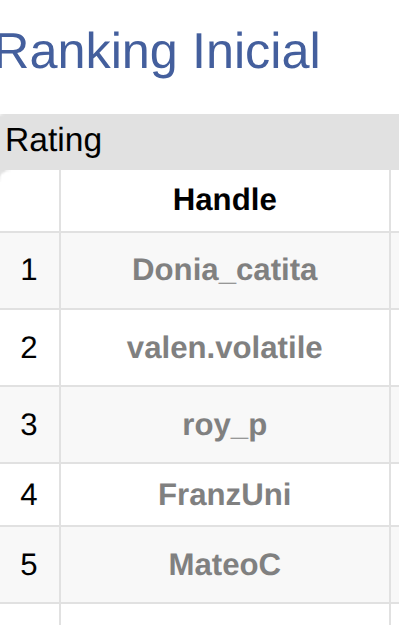
\includegraphics[width=0.7\textwidth,keepaspectratio]{img/inicial-1.png}
        \column{0.5\textwidth}
        \centering
        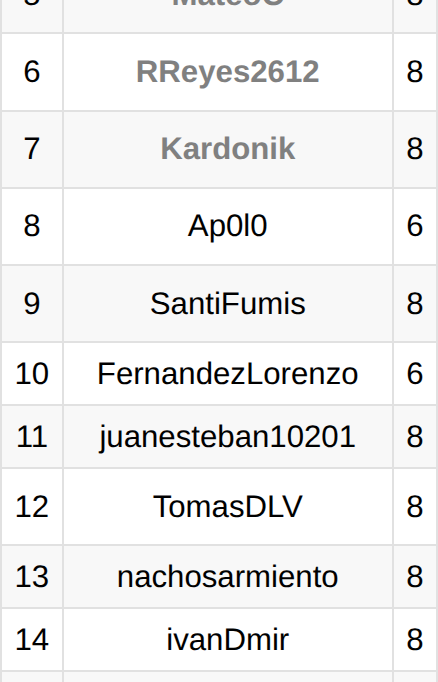
\includegraphics[width=0.7\textwidth,keepaspectratio]{img/inicial-2.png}
    \end{columns}
\end{frame}

\begin{frame}{Ranking Avanzado}
    \begin{columns}
        \column{0.5\textwidth}
        \centering
        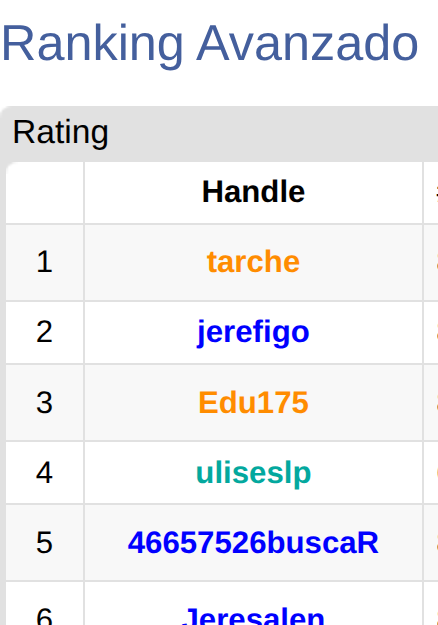
\includegraphics[width=0.7\textwidth,keepaspectratio]{img/avanzado-1.png}
        \column{0.5\textwidth}
        \centering
        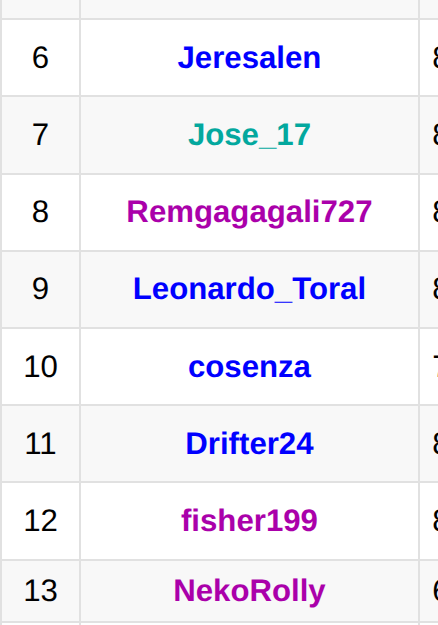
\includegraphics[width=0.7\textwidth,keepaspectratio]{img/avanzado-2.png}
    \end{columns}
\end{frame}


\section{y que hago con todo lo que aprendi?}

\begin{frame}{y que hago con todo lo que aprendi?}
    \begin{center}
        
\includegraphics[width=0.45\textwidth,keepaspectratio]{img/qr-code-aapc.png}

        \vspace{0.5cm}
        {\small
        \textbf{¡Hacete socio/a de la AAPC!}\\
        Apoyá la programación competitiva en Argentina.\\
        \href{https://icpc.com.ar/socios/}{https://icpc.com.ar/socios/}
        }
    \end{center}
\end{frame}

\begin{frame}{Maratona Feminina de Programação (MFP) - Información General}
\begin{center}

\includegraphics[width=0.2\textwidth,keepaspectratio]{img/mfp_logo.jpeg}

\vspace{0.3cm}

\Large
\textbf{Maratona Feminina de Programação}

\vspace{0.2cm}

\normalsize
\textbf{Competencia exclusiva para mujeres en programación}

\vspace{0.3cm}

\begin{itemize}
\item \textbf{Objetivo:} Promover la participación femenina en programación competitiva
\item \textbf{Formato:} Competencia individual o en equipos
\item \textbf{Duración:} 5 horas de competencia intensiva
\item \textbf{Lenguajes:} C/C++, Python, Java, entre otros
\item \textbf{Organización:} Sociedad Brasileña de Computación (SBC)
\end{itemize}

\vspace{0.3cm}

\textbf{¡Una oportunidad única para demostrar tu talento!}

\vspace{0.2cm}

\small
\url{https://www.instagram.com/mfp.sbc}
\end{center}
\end{frame}

\begin{frame}{Maratona Feminina de Programação (MFP) - Beneficios y Participación}
\begin{center}
\Large
\textbf{¿Por qué participar en MFP?}

\vspace{0.1cm}

\normalsize
\begin{itemize}
\item \textbf{Networking:} Conoce a otras programadoras apasionadas
\item \textbf{Desarrollo:} Mejora tus habilidades de resolución de problemas
\item \textbf{Visibilidad:} Demuestra tu talento en la comunidad
\item \textbf{Mentoría:} Acceso a mentoras experimentadas
\item \textbf{Oportunidades:} Puertas abiertas a competencias internacionales
\end{itemize}

\vspace{0.1cm}

\textbf{¡Rompe barreras y construye tu futuro en tecnología!}

\vspace{0.2cm}

\small
\url{https://www.instagram.com/mfp.sbc}
\end{center}
\end{frame}

\begin{frame}{Torneo Argentino de Programación (TAP) - Información General}
\begin{center}

\includegraphics[width=0.2\textwidth,keepaspectratio]{img/tap_logo.png}

\vspace{0.1cm}

\Large
\textbf{16º Torneo Argentino de Programación 2026}

\normalsize
\textbf{Sábado 29 de agosto de 2026}

\vspace{0.1cm}

\begin{itemize}
\item \textbf{Competencia:} 5 horas de duración
\item \textbf{Equipos:} 3 personas por equipo (1 PC)
\item \textbf{Lenguajes:} C/C++, Python, Java o Kotlin
\item \textbf{Requisito:} Ser estudiante de educación superior en Argentina
\item \textbf{Clasificación:} Para la Regional Sudamérica-Sur (SAS)
\end{itemize}

\textbf{¡Inscripciones próximamente!}

\small
\url{https://aapc.org.ar/tap/}
\end{center}
\end{frame}

\begin{frame}{Torneo Argentino de Programación (TAP) - Sedes de Competencia}
\begin{center}
\Large
\textbf{Múltiples sedes en todo el país}

\vspace{0.5cm}

\normalsize
Al igual que todos los años, el TAP se compite de forma simultánea en diversas universidades nacionales e institutos de toda la Argentina.

\vspace{0.5cm}

\begin{block}{¡Tu universidad puede ser sede!}
    Solo se requiere una conexión a internet estable, laboratorios de computación o aulas acondicionadas, y un docente/organizador local responsable.
\end{block}

\vspace{0.5cm}

Para consultar la lista completa y actualizada de sedes habilitadas:

\vspace{0.2cm}
\small
\url{https://aapc.org.ar/tap/}
\end{center}
\end{frame}

\begin{frame}{Regional Sudamérica-Sur}
\begin{center}
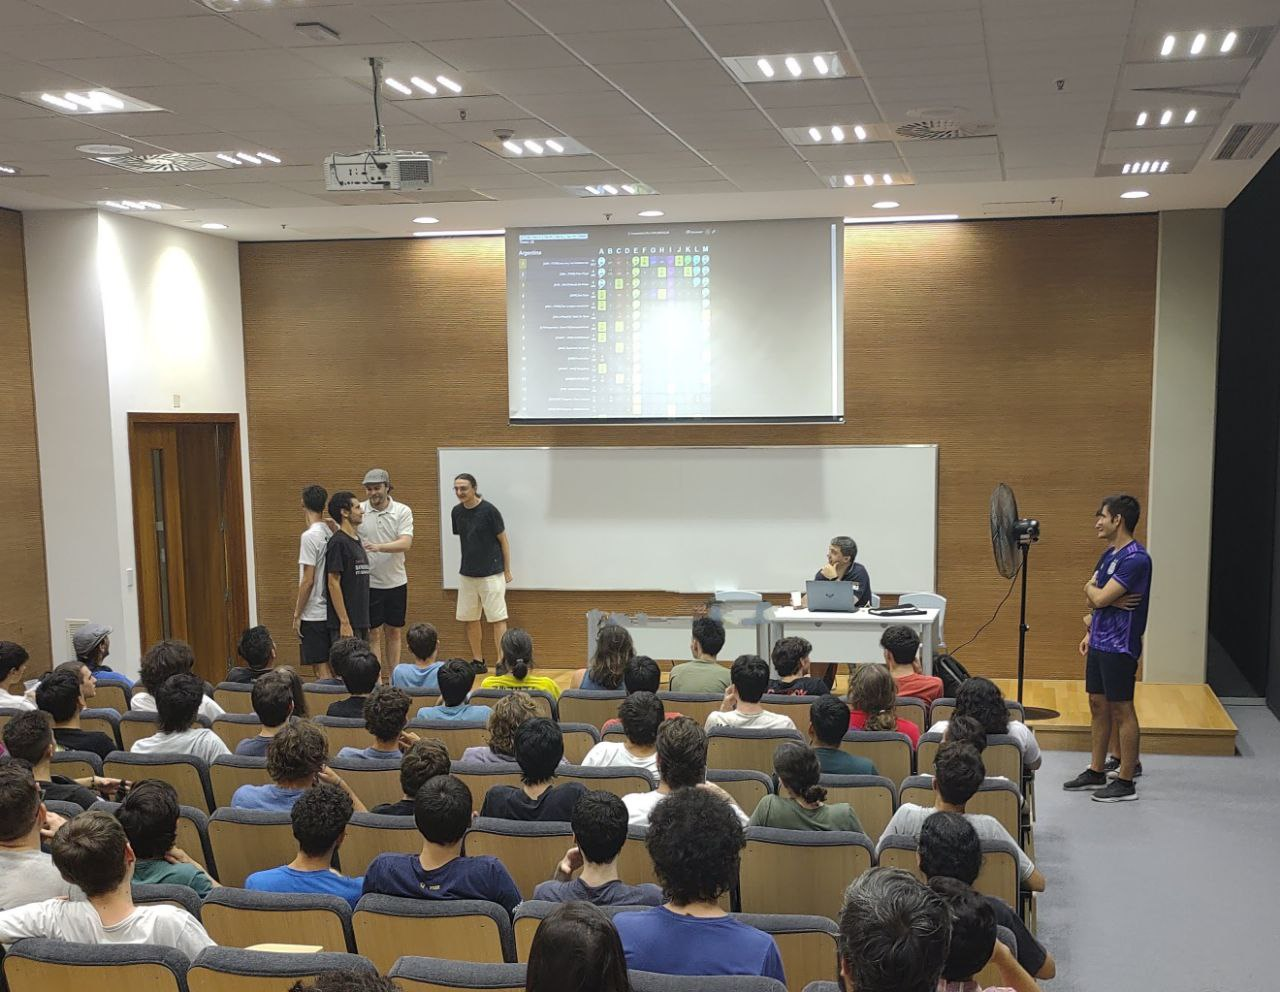
\includegraphics[width=0.3\textwidth,keepaspectratio]{img/regional_logo.jpg}

\vspace{0.2cm}

\Large
\textbf{Regional Sudamérica-Sur 2026}

\vspace{0.1cm}

\normalsize
\textbf{Sábado 7 de noviembre de 2026} \\
\small{Sede prevista: Ciudad de Santa Fe, Argentina}

\vspace{0.2cm}

\begin{itemize}
\item \textbf{Participantes:} Equipos clasificados del TAP y otros países
\item \textbf{Países:} Argentina, Chile, Uruguay, Paraguay, Bolivia
\item \textbf{Formato:} 5 horas de competencia intensiva
\item \textbf{Premio:} Clasificación a PDA 2027 (Monterrey)
\end{itemize}

\vspace{0.1cm}

\textbf{¡El siguiente paso después del TAP!}

\small
\url{https://icpc.com.ar/regional-latinoamericana}
\end{center}
\end{frame}

\begin{frame}{Presentación Programadores de América 2027}
\begin{center}
\Large
\textbf{Video de Presentación}

\vspace{0.6cm}

\normalsize
¡Te invitamos a ver el video oficial de presentación de la competencia!

\vspace{0.4cm}

\href{https://www.facebook.com/share/v/18C9toisj2/}{
\includegraphics[width=0.45\textwidth,keepaspectratio]{pda_logo_new.png}}

\vspace{0.4cm}
\small
Link al video: \url{https://www.facebook.com/share/v/18C9toisj2/}
\end{center}
\end{frame}

\begin{frame}{Programadores de América 2027}
\begin{center}

\vspace{0.2cm}

\normalsize
\textbf{Monterrey, México, Marzo 2027}

\vspace{0.2cm}


\includegraphics[width=0.45\textwidth,keepaspectratio]{pda_logo_new.png}

\vspace{0.3cm}

\begin{itemize}
\item \textbf{Competencia:} Final continental de programación
\item \textbf{Participantes:} Mejores equipos de Latinoamérica
\item \textbf{Formato:} 5 horas de competencia intensiva
\item \textbf{Cupos:} 80 cupos (el doble que en 2026, solo por esta edición)
\item \textbf{Premio:} Clasificación a la Final Mundial ICPC 2027
\end{itemize}

\vspace{0.2cm}

\textbf{¡La meta final de todo programador competitivo!}

\small
\url{https://icpc.global}
\end{center}
\end{frame}

\begin{frame}{¿Training Camp 2027?}
\begin{center}
\Large
\textbf{Sede a definir}

\vspace{0.6cm}

\normalsize
Si tu universidad o facultad está interesada en ser sede del próximo Training Camp Argentina 2027, ¡queremos saber de vos!

\vspace{0.5cm}

\begin{block}{Contacto y Postulaciones}
    Pueden ponerse en contacto directamente con los organizadores del TC o escribir a la AAPC para postular a su institución.
\end{block}

\vspace{0.8cm}
\textbf{¡Hagamos crecer la programación competitiva juntos!}
\end{center}
\end{frame}


\section{Gracias a todos}

% TODO: Update lecturers list for 2026
\begin{frame}{Gracias Disertantes}
    \begin{itemize}
        \item Federico Quijada
        \item Mariano Feresin
        \item Agustín Santiago Gutiérrez
        \item Mateo Carranza Velez
        \item Federico Bersano
        \item Lautaro Lasorsa
        \item Franco De Rico
        \item Ivo Pajor
        \item Sebastián Mestre
        \item Matías Fluxa
        \item Luis Santiago Re
        \item Eduardo Carranza Velez
        \item Joaquín Inama
    \end{itemize}
\end{frame}

% TODO: Update setters list for 2026
\begin{frame}{Gracias Setters}
    \begin{itemize}
        \item {\color{orange} MateoCV}
        \item {\color{orange} elsantodel90}
        \item {\color{orange} lsantire}
        \item {\color{orange} Heibor}
        \item {\color{orange} MarcosK}
        \item {\color{orange} matramos}
        \item {\color{orange} Guty}
    \end{itemize}
\end{frame}

% TODO: Update volunteers list for 2026
\begin{frame}{Gracias Voluntarios}
    \begin{center}
        \Large
        Vicky, Marti, Naza y Fiebre (Gonza).

        \vspace{1cm}

        \normalsize
        Hacedores del coffee-break y ayuda para que todo salga bien.
    \end{center}
\end{frame}

\begin{frame}{Gracias UNLP -- Facultad de Informática}
    \begin{center}
        
\includegraphics[width=0.8\textwidth,keepaspectratio]{unlp_informatica.png}

        \vspace{0.5cm}
        Equipo de Soporte, Mantenimiento, Limpieza, etc.
    \end{center}
\end{frame}

\begin{frame}{Gracias a ustedes}
    \begin{center}
        \includegraphics[width=0.7\textwidth,keepaspectratio]{cierre_final.jpg}

        \vspace{0.5cm}
        nos vemos en TC 2027?
    \end{center}
\end{frame}

\end{document}
